\documentclass[c,compress]{beamer}
\usetheme{Boadilla}
\usecolortheme{dolphin}
\renewcommand{\baselinestretch}{1.5} 
\usepackage{cite}
\usepackage{amsmath,amssymb,amsfonts}
\usepackage{algorithmic}
\usepackage{graphicx}
\usepackage{diagbox}
\usepackage{array,multirow}
\usepackage{minted}
\usepackage[T1]{fontenc}
% \usepackage{eucal}
\newcommand*{\textcal}[1]{%
  % family qzc: Font TeX Gyre Chorus (package tgchorus)
  % family pzc: Font Zapf Chancery (package chancery)
  \textit{\fontfamily{qzc}\selectfont#1}%
}

\usepackage{hyperref}
\hypersetup{
	pdftitle={JournalClub_HNN},
   colorlinks=false,
   citecolor=blue,
   linkcolor=black,
   urlcolor=blue
}

\usefonttheme{structurebold}
\setbeamercolor{title}{fg=black}
\setbeamercolor{frametitle}{fg=black}
\title{Reservoir Computing}
\author{Anil Radhakrishnan}
\institute{University of Illinois}
\date{ML Journal Club, June 4 2020 }
\addtobeamertemplate{navigation symbols}{}{%
    \usebeamerfont{footline}%
    \usebeamercolor[fg]{footline}%
}
\definecolor{blue(pigment)}{rgb}{0.2, 0.2, 0.6}
\def\bsq{\color{blue(pigment)} $\blacksquare$ \color{black}}



\begin{document}

\frame{\titlepage}

% Slide 1
\begin{frame}{Motivation\\\rule{10.5cm}{0.5pt}} \label{Motiv}
\bsq Classical RNN are difficult to train by gradient descent due to several reasons:
\begin{itemize}
    \item A high temporal complexity slowing down the training process
    \item Instability and bifurcations
    \item Vanishing gradient
    \item Local minimas
\end{itemize}
\bsq Reservoir Computing aims to separate the parts where computing in done and the output layer where learning is done

\end{frame} 
% Slide 2
\begin{frame}{What is it\\\rule{10.5cm}{0.5pt}} \label{def}
\bsq Essentially a recurrent neural network with loosely connected hidden layer or \textbf{reservoir}\\
\bsq The main idea is to :
\begin{enumerate}
    \item Drive a random, large, fixed recurrent neural network with the input signal, thereby inducing in each neuron within this reservoir network a nonlinear response signal
    \item Combine a desired output signal by a trainable linear combination of all of these response signals. 
\end{enumerate}

\end{frame}

% Slide 3
\begin{frame}{Why this works\\\rule{10.5cm}{0.5pt}} \label{keys}
\bsq A simple way to learn a feed-forward net is to make early layers random and fixed\\
\bsq A big random expansion of input vectors can help.($\sim$SVM)\\
\bsq Output weights change much more rapidly than ones in the hidden layer$\rightarrow$ \href{http://citeseerx.ist.psu.edu/viewdoc/download?doi=10.1.1.161.9279&rep=rep1&type=pdf}{BackPropagation-Decorellation(BPDC)}

\end{frame} 



% Slide 2
\begin{frame}{Creating a Reservoir\\\rule{10.5cm}{0.5pt}} \label{EchoState}
\bsq Set the hidden→hidden weights so that the length of the activity vector stays about the same after each iteration( $\rho(W) <\approx 1$)\\
    - This allows the input to \textbf{echo} around the network for a long time\\
\bsq Use sparse connectivity to create lots of loosely coupled oscillators\\
\bsq The scale of input→hidden connections should be chosen carefully to not wipe out past information\\
\bsq The Reservoir will asymptotically wash out any information from the initial conditions\\
\end{frame}


% Slide 4
\begin{frame}{Comparing to traditional RNN\\\rule{10.5cm}{0.5pt}} \label{slide4}
\begin{figure}
    \centering
    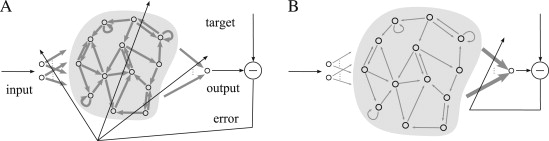
\includegraphics[width=0.95\paperwidth]{RNN_ESN.png}
    {A. Traditional gradient-descent-based RNN training methods adapt all connection weights (bold arrows), including input$\rightarrow$RNN, RNN$\rightarrow$internal, and RNN$\rightarrow$output weights. \\B. In Reservoir Computing, only the RNN$\rightarrow$output weights are adapted.}
    \label{fig:my_label}
\end{figure}
\end{frame}

%Silde 7
\begin{frame}{Network Schematic\\\rule{10.5cm}{0.5pt}} \label{slide7}
\begin{figure}
    \centering
    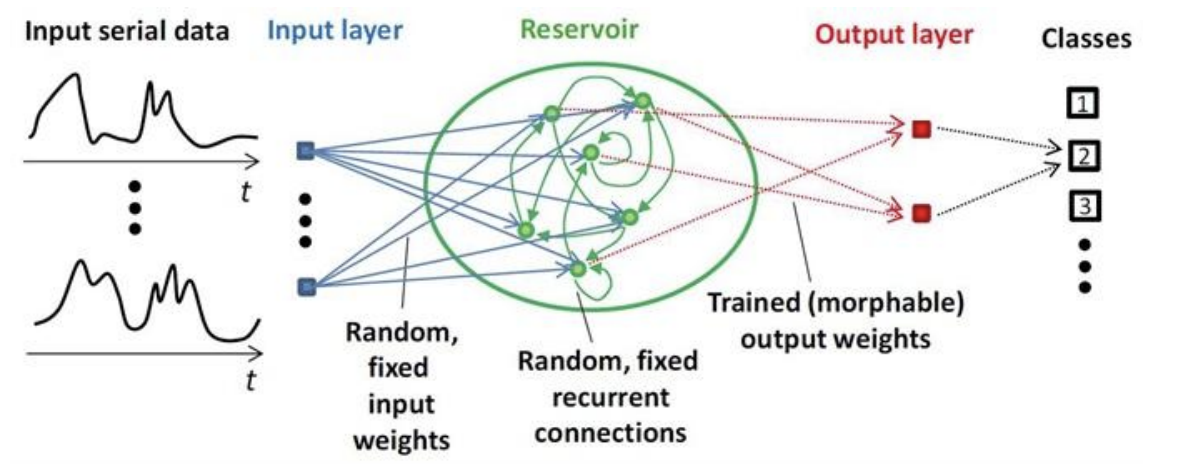
\includegraphics[width=0.95\linewidth]{training.png}
    \label{fig:amazon}
\end{figure}

\end{frame}

% Slide 6
\begin{frame}{Results\\\rule{10.5cm}{0.5pt}} \label{slide6}
\begin{figure}
    \centering
    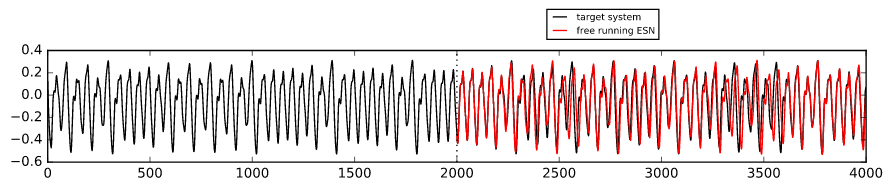
\includegraphics[width=0.85\linewidth]{ESN_mackey_glass.png}
    \\Predicting chaotic time series --- Mackey-Glass equation
    \label{fig:mackey}
\end{figure}
\[
\frac{dx}{dt} = \beta \frac{ x_{\tau} }{1+{x_{\tau}}^n}-\gamma x, \quad \gamma,\beta,n > 0
\]
\end{frame}

%Silde 7
\begin{frame}{Results\\\rule{10.5cm}{0.5pt}} \label{slide7}
\begin{figure}
    \centering
    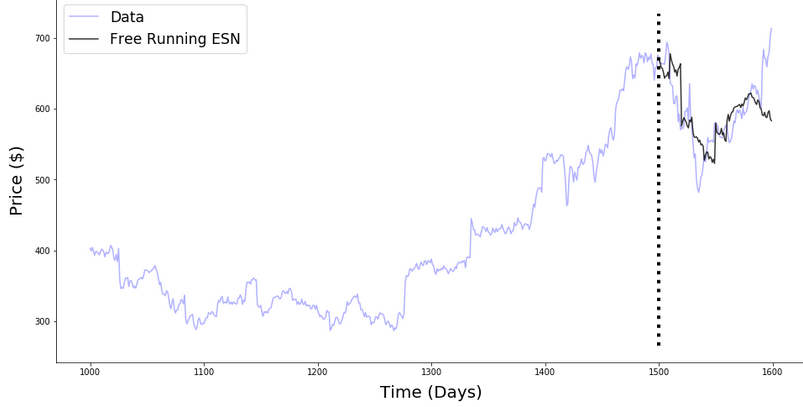
\includegraphics[width=0.80\linewidth]{amazon_predict_esn.png}
    \\ Predicting Amazon stock prices 
    \label{fig:amazon}
\end{figure}

\end{frame}

%Silde 8
\begin{frame}{Utility\\\rule{10.5cm}{0.5pt}} \label{slide7}
\bsq Benefits 
\begin{itemize}
    \item Can be trained very fast because its basically fitting a linear model
    \item illustrates the importance of sensible weight initialization
    \item Impressive 1-d time series modelling
\end{itemize}
\bsq Drawbacks 
\begin{itemize}
    \item Needs many more hidden units for a given tasks than an RNN that learns the hidden→hidden weights
\end{itemize}
\end{frame}


% Slide 8
\begin{frame}{Other ideas and implementations\\\rule{10.5cm}{0.5pt}} \label{slide8}
\bsq \href{http://prg.cs.umd.edu/research/reservoir_files/reservoir.pdf}{Generalized learning with reservoir computing}\\
\bsq \href{https://iopscience.iop.org/article/10.35848/1347-4065/ab8d4f}{Physical Reservoirs}\\
\bsq \href{https://www.intechopen.com/books/intelligent-system-and-computing/the-novel-applications-of-deep-reservoir-computing-in-cyber-security-and-wireless-communication}{Reservoir computing in cyber security and wireless communication}\\
\bsq \href{https://royalsocietypublishing.org/doi/10.1098/rstb.2018.0377#d3e3070}{RC for understanding evolutionary biology}\\
\bsq \href{https://arxiv.org/pdf/1712.04323.pdf}{DeepESN}
\end{frame}


% Slide 9
\begin{frame}{Concluding remarks\\\rule{10.5cm}{0.5pt}} \label{slide9}
A randomly generated fixed RNN with only a linear readout outperforming state of the art RNN training method has several consequences:
\begin{itemize}
    \item We need better techniques to train RNNs well
    
    \item Classical RC methods are not yet exploiting the full potential of RNNs, since they use a random RNN and a linear readout
    
    \item The separation between the RNN reservoir and the readout provides a platform to try out different RNN adaptation methods in the reservoir to see improvements over a random RNN.
    
\end{itemize}

\end{frame}


\end{document}